\chapter{Design and Implementation of Porting Basic Components of Xen Split Driver Model\label{cha:chapter5}}
For porting Xen split driver model, three major components i.e. Grant tables, Event channels and Xenstore would be modified to use static memory and PHIDIAS xcore and capability feature. In this section, design and implementation of applying \textit{\textbf{Principle of Staticity}} of PHIDIAS to Xen I/O drivers will be discussed.

\section{Porting Xen I/O Emualation Layer to PHIDIAS\label{sec:memstatic}}
Porting work for necessary components of XEN's split driver model is explained in the following sections.

\subsection{Porting Shared Information Pages\label{sec:sharedinfo}}
Shared info page is used to share virtual machine state with Xen hypervisor. It includes information about virtual CPU (vCPU) state, event channels and wall clock time information. Each guest allocates a zerod page for shared info page from kernel and registers it with Xen hypervisor through a hypercall. In our case, a static memory range has been configured to allocate shared info pages. These pages are shared between guests instead with the PHIDIAS hypervisor. The size of this static memory is dependent upon the total number of configured guests in system. Each guest obtains its share info page from this static contiguous memory range using its domain ID defined in Linux configuration file (CONFIG\_XEN\_DOM\_ID). Dom0 with id 0 initializes the entire range with zeros. The shared info page is mapped in linux guest as un-cached so that other guests would get the consistent view of each other's shared information. Figure \ref{sharedinfo} shows the approach of implementing shared info pages for two guests in PHIDIAS.
\begin{figure}[!htbp]
	\centering
	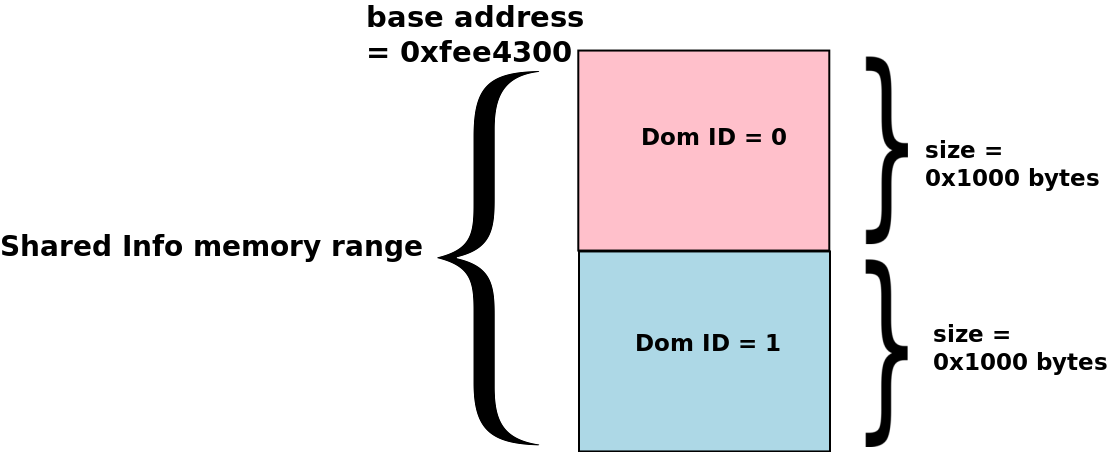
\includegraphics[width=10cm]{sharedinfo}
	\caption{Basic approach of implementation of shared info pages in PHIDIAS for two guests}
	\label{sharedinfo}
\end{figure}

\section{Design of Porting Grant Tables\label{sec:granttablesstatic}}
As described in \ref{sec:granttables}, grant tables are a mechanism for sharing memory pages across domains. Each guest allocates pages for grant tables and shares them with Xen hypervisor through a hypercall. By design, Xen does not support swapping which means that even unused part of allocated memory to a guest will be not used by other guests. To solve this problem, Xen uses \textbf{ballooning}. Ballooning is way of dynamically increasing or decreasing size of allocated memory from hypervisor's memory pool. Memory visible to each guest can be configured in Xen at boot time. For Dom0, it could be specified in grub configuration file and for domU, it is specified in XL tool's guest configuration file. If the guest uses less memory than configured amount, it can return nused blocks of memory to hypervisor. However, guest can not retrieve more memory through ballooning than its maximum configured amount of memory. Memory allocated to unprivileged guests is taken from Dom0 memory pool and hence it Dom0 memory balloon's down every time a new guest is started.
\\
\\
For the current work, Xen balloon driver has been disabled in Linux guest kernel using configuration option CONFIG\_XEN\_BALLOON. In the native code of xen domains, ballooning is used to allocate pages for grant tables, XenBus ring buffers and netback driver for mapping packets received from netfront. In our ported setup, it has been replaced by defining two globally shared readable/writable memory ranges statically in PHIDIAS configuration option of guests. One memory range is defined to allocate static memory for grant table frames while the other is defined to be used by all split drivers for establishing communication for I/O virtualization. Required pages are allocated from these two memory ranges and mapped un-cached in address spaces of guests.

\subsection{Static Memory for Grant Frames\label{sec:granttablesframes}}
In Xen, maximum number of grant frames is defined to be 32. For the current thesis, since two guests were used for testing, a total of 64 contiguous pages had been configured for grant tables usage. Each guest uses 32 pages for its own grant table implementation and accesses other guests' grant table by mapping these into its address space un-cached. For performing operations on grant tables, each guest gets the reference of unused entry from grant table and updates it with its domain ID, shared frame number and desired flags. The guest then sends the obtained grant reference through ring buffers to the other guest. In native Xen domains, hypercalls are used to perform grant operations i.e. granting access to remote domain, mapping, transferring and copying pages across domains. In ported static setup, guest had access to remote's domains grant tables by mapping those directly into its address space. Figure \ref{grant_table} shows the configuration of grant table static memory range for two guests in PHIDIAS.
\begin{figure}[!htbp]
	\centering
	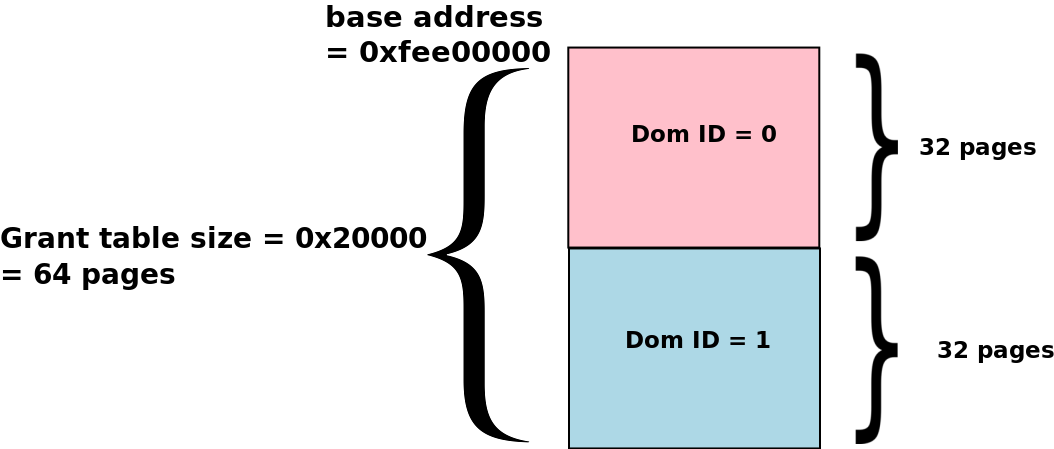
\includegraphics[width=10cm]{grant_table}
	\caption{Static memory configuration for grant table in PHIDIAS for two guests}
	\label{grant_table}
\end{figure}

\subsection{Static Memory for I/O Split Drivers Usage\label{sec:splitdriverusage}}
I/O Split drivers of Linux guests allocates pages using kernel APIs for the allocation of page frames and share with other guests via grant table hypercalls. In order to use the same Linux page allocation APIs and keep changes in split drivers as minimum as possible, a new memory zone named \textbf{ZONE\_XEN} had been added in Linux kernel. A static globally shared memory of size 8192KB has been allocated in PHIDIAS from which each guest can allocate its respective zone. The size of zone for each guest was set to 4096 KB i.e. 1024 pages. Each guest obtained the starting address of its zone using base address configured in PHIDIAS for zone memory range and its domain ID as shown in listing \ref{list_zone}.
\\
\begin{lstlisting}[caption=Code snippet for calculating start address of guest ZONE\_XEN, label={list_zone}]
    xen_zone_size = 0x400000;
    xen_zone_start_addr = 0xfef00000 + (CONFIG_XEN_DOM_ID * xen_zone_size);

\end{lstlisting}
Figure \ref{zone_xen} shows the memory configuration for areas of ZONE\_XEN for two guests in PHIDIAS.
\begin{figure}[!htbp]
	\centering
	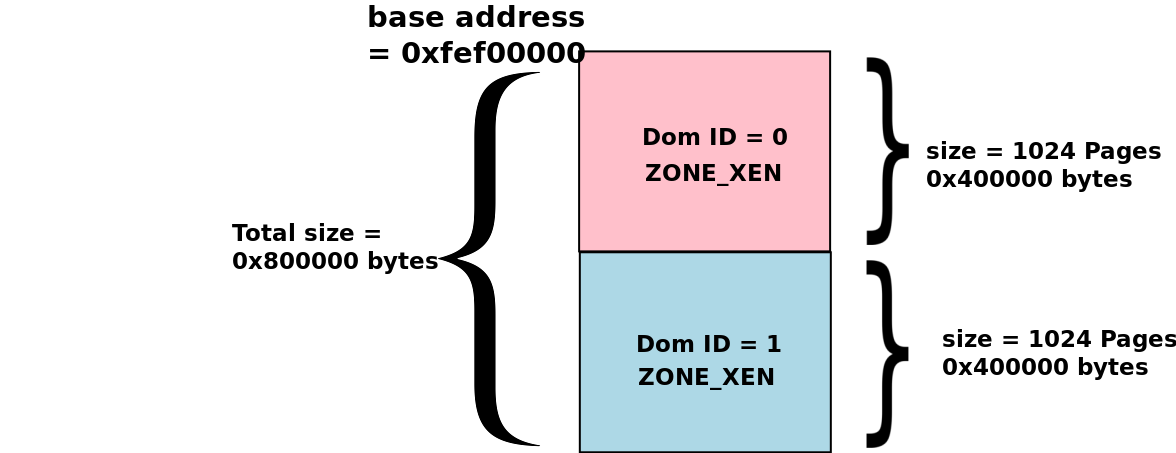
\includegraphics[width=10cm]{zone_xen}
	\caption{Static memory configuration for ZONE\_XEN in PHIDIAS for two guests}
	\label{zone_xen}
\end{figure}

Each guest knows about the address range of other guests ZONE\_XEN. In order to access remote guests pages allocated from their ZONE\_XEN, each guest maps the areas of other guests zones into its address space during its initialization and creates a hash table of virtual addresses of mapped pages indexed with physical page frame numbers. This hash table was implemented for ported split drivers for two reasons:

\begin{itemize}
	\item To speed up the process of finding mapped virtual address of remote's guest shared page using the physical frame numbers obtained from remote guest's grant table which are already mapped as explained in \ref{sec:granttablesframes}.
	\item Function ioremap can not be called in interrupt context which is the case of mapping shared pages through grant tables in split drivers for most of the scenarios.
\end{itemize}

Figure \ref{hash_table} shows the basic structure of hash table for mapping remote guest's physical frame numbers of shared pages to mapped virtual addresses in local address space.

\begin{figure}[!htbp]
	\centering
	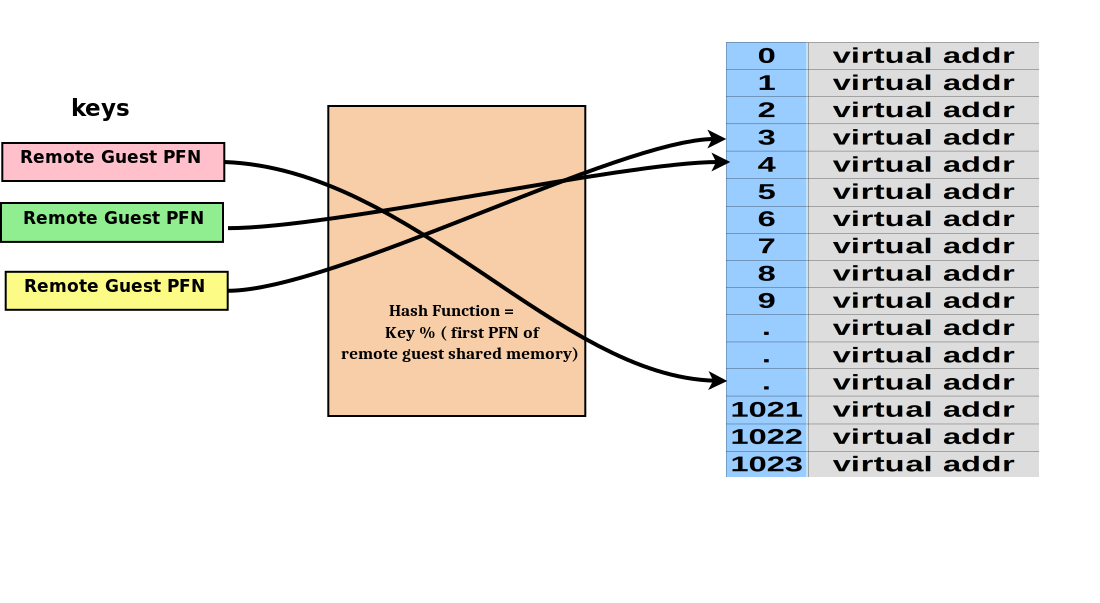
\includegraphics[width=10cm]{hash_table}
	\caption{Structure of hash table used for accessing remote guest shared pages of zone xen}
	\label{hash_table}
\end{figure}


\section{Design of Porting Event Channels\label{sec:eventstatic}}
As explained in section \ref{sec:eventchannel}, event channels are used to send asynchronous notifications among guests in Xen. On ARM, software generate interrupts (SGI) are used for interprocessor interrupts. There are 16 SGI available on ARM architecture. In Xen guests, there is a common interrupt handler \textbf{xen\_arm\_callback} for handling notifications from remote guests via event channels. Xen guest uses PPI 31 for event IRQ and has a an interrupt property in its hypervisor node of flattened device tree provided to it by hypervisor as shown in listing \ref{xen_node}.
\\
\\
\begin{lstlisting}[caption=Xen Hypervisor node in hi6220 flattened device tree, label={xen_node}]
 hypervisor {
     compatible = "xen,xen", "xen,xen-4.7"; //version of the Xen ABI 
     reg = <0xb0000000 0x20000>;            // Grant table memory area 
     interrupts = <1 15 0xf08>;             //event notifications IRQ
 };

\end{lstlisting}
In PHIDIAS, SGIs are used to send interprocess interrupts using its \textbf{xcore mechanism}. First 6 SGI interrupts are used by Linux kernel. Our port could use one from the remaining SGIs for registering \textbf{xen\_arm\_callback} handler for Xen event IRQ. However, in Linux kernel version 4.11\_rc2 used in current work, handle\_IPI function used for handling SGIs only handles first 6 SGIs already registered by Linux kernel. For remaining SGIs, it shows a default warning of \textit{Unknown IP}. To handle this, some modifications were made in IPI handling code of Linux kernel. For SGIs greater than 5, modified IPI handling function checked whether some handler is registered for incoming interrupt and then called the registered handler if found any. A kernel level API for registering IPI handler for SGIs was added. Web source \cite{smp} has been used as a reference for implementing generic API for registering custom IPI handlers.
\\
\\
SGI 9 had been used for Xen events in PHIDIAS for interdomain communication. 2-level event channel support had been ported which used two-level bitmap to speed searching. The first level is a bitset of words which contain pending event bits.  The second level is a bitset of pending events themselves. All hypercalls in Xen guests were replaced with local guest's kernel code working on shared memory and IPIs. 

\subsection{Static Memory Allocation for Event Domains Pages \label{sec:eventsdomains}}
Xen hypervisor maintains a structure for each event per domain which stores necessary information e.g. VCPU for local delivery notification, event channel type, port number and priority etc. When a guest issues hypercall to send an event to remote guest, Xen hypervisor uses this structure to find remote domain ID and remote port and injects interrupt into destination guest. 
\\
\\
In current work, all maintenance of event domain structures and triggering of IPI had been moved into Xen's guest domain. For remote sharing of event channel structures of guests, a static globally shared memory named \textbf{event\_domains} has been allocated and mapped to guests' domains. In our implementation, the number of event channels each guest could support was limited to the amount of event domain structures that a single page could hold. Each guest had access to remote guest's event domain page containing corresponding event domain structures and could write its domain id and local event port into them while binding interdomain event channels. Figure \ref{event_domains} shows the basic structure of sharing event domains information in PHIDIAS for two guests.

\begin{figure}[!htbp]
	\centering
	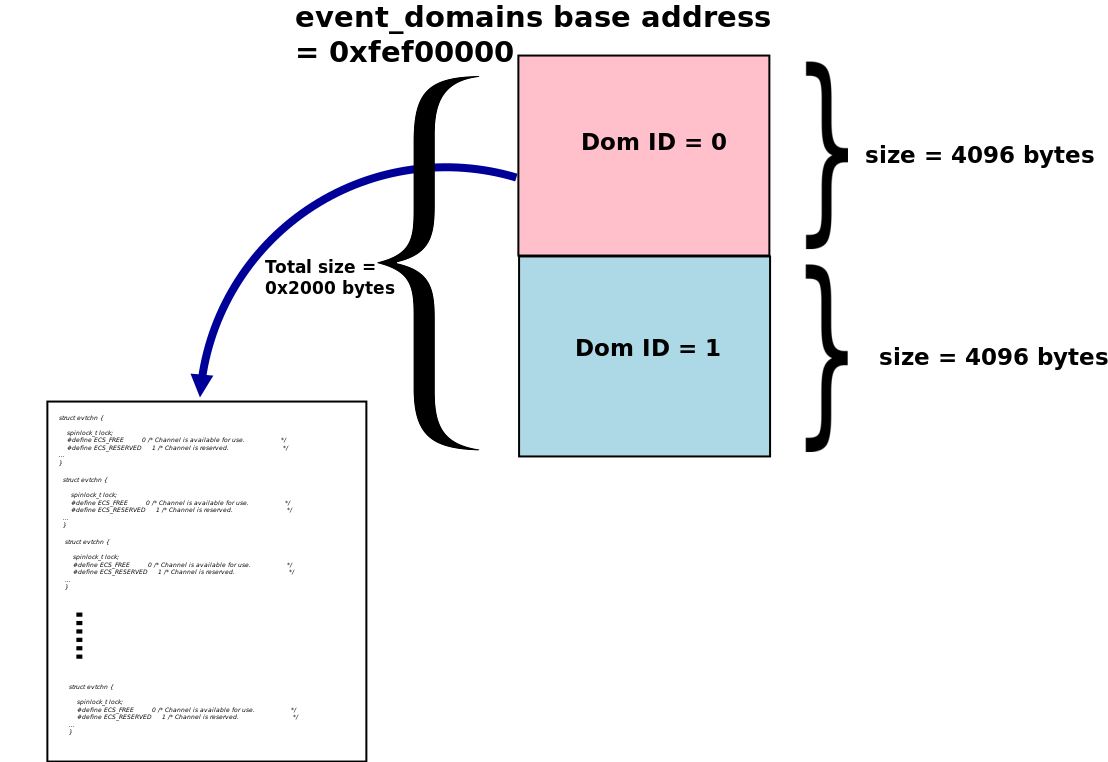
\includegraphics[width=10cm]{event_domains}
	\caption{Basic structure of sharing event domains information in PHIDIAS for two guests}
	\label{event_domains}
\end{figure}

\subsection{Adding Capabilities for IPI in PHIDIAS \label{sec:eventsdomains}}
In case of split driver model of Xen, guests use event channels in two scenarios:
\begin{itemize}
	\item Sending event notifications between Xenstore userspace application and guest's  paravirtualized I/O driver behaving as intradomain events.
	\item Sending event notification between two frontend and backend of split drivers behaving as interdomain events.
\end{itemize}
For the above two types of events, two capabilities had been added in guest configuration on PHIDIAS as shown in listing \ref{cap}.\\

\begin{lstlisting}[caption=Capabilities added for event notifications in guest configuration on PHIDIAS, label={cap}]
For Dom0 Linux guest 1
      <cap type="ipc" target_xref="linux2" param="0x9" /> 
      <cap type="ipc" target_xref="linux1" param="0x9" /> 
For DomU Linux guest 2
      <cap type="ipc" target_xref="linux1" param="0x9" /> 
      <cap type="ipc" target_xref="linux2" param="0x9" /> 
\end{lstlisting}

Both capabilities had type \textbf{ipc}. First capability had index 0 with destination selected to be remote guest and second capability had index 1 with destination chosen to be itself. First capability was used for \textbf{interdomain events} and second capability emulated \textbf{intradomain events}. Both these capabilities triggers SGI 9 for xen events in linux guests.

\section{Design of Porting Xenstore\label{sec:xenstorestatic}}
As explained previously in section \ref{sec:xenstore}, each guest of Xen shares a page for xenstore request and response ring buffers with Xenstore userspace application. It also binds an event channel with Xenstore application to send event notifications. Xenstore userspace application talks with Xen guests through \textbf{\textit{Xen filesystem xenfs}} driver which mounts files for communication between Xen guests and userspace applications. Out of these files, following two are used for communication between Xenstore and Xen Dom0 guest:
\begin{itemize}
	\item xsd\_kva for mapping guest's page used for xenstore interface in userspace
	\item xsd\_port for getting an unbound port number of the guest event channel used for binding it with a event port in userspace application i.e.Xenstore daemon. 
\end{itemize}
For unprivileged guests of Xen, Dom0 controls their creation and performs management through Domain control hypercalls. While creation of DomU,a xenstore interface page and an unbound event channel are allocated which are introduced into xenstore daemon through Xen XL tool. DomU gets that allocated page for mappingit into its address space and the xenstore event channel with the help of hypercalls during its initialization.
\\
\\
In our current work, since no XL tool had been ported and Dom0 did not control creation of DomU guests, DomU xenstore page and event channel number was added manually. A similar file interface had been exposed to userspace by Dom0 which was used to map DomU xenstore page into Xenstore daemon application as shown in listing \ref{xvd_foreign}. Two globally shared static pages were allocated for xenstore interfaces of guests in PHIDIAS  as shown in Figure \ref{xenstore-Page}. For event channel of DomU used with xenstore daemon, hard-coded DomU's event port number 1 was used. Mechanism for introducing DomU to Xenstore daemon with hypercalls and XL tool was replaced with by manually introducing creation of DomU connection into xenstore daemon code.

\begin{figure}[!htbp]
	\centering
	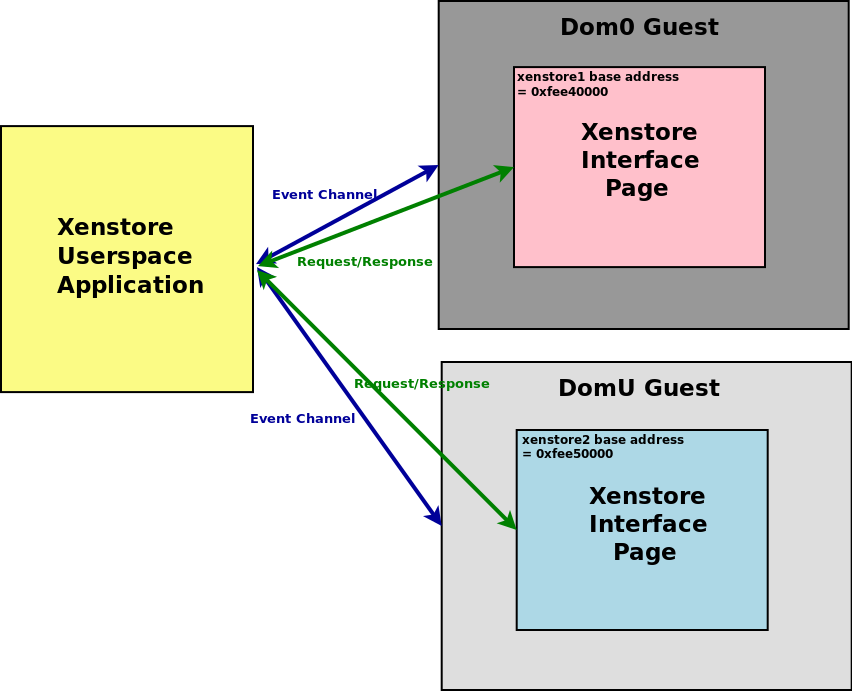
\includegraphics[width=10cm]{xenstore-Page}
	\caption{Communication between Xenstore application and Guests in PHIDIAS}
	\label{xenstore-Page}
\end{figure}


\begin{lstlisting}[caption=Added file interface for mapping DomU xenstore interface page into userspace in drivers/xen/xenfs/xenstored.c file, label={xvd_foreign},frame=single,style=base]
...
static int @ xsd_foreign_kva_mmap @(struct file *file, struct vm_area_struct *vma)
{
    size_t size = vma->vm_end - vma->vm_start;

    if ((size > PAGE_SIZE) || (vma->vm_pgoff != 0))
        return -EINVAL;
        
    vma->vm_page_prot = pgprot_noncached(vma->vm_page_prot);

    if (io_remap_pfn_range(vma, vma->vm_start,
                           0xfee45000 >> XEN_PAGE_SHIFT,
                           size, vma->vm_page_prot))
        return -EAGAIN; 

    return 0;
}

const struct file_operations xsd_kva_foreign_file_ops = {
    .open = xsd_foreign_kva_open,
    .mmap = @xsd_foreign_kva_mmap@,
    .read = xsd_read,
    .release = xsd_release,
};

...
\end{lstlisting}



